\documentclass[conference]{IEEEtran}
\usepackage{graphicx}
\usepackage{booktabs}
\usepackage{amsmath}
\usepackage{url}
\usepackage[hidelinks]{hyperref}

\begin{document}

\title{Small Language Models from Scratch: Pre-training, Instruction Fine-Tuning and Linear Attention on a Single GPU}

\author{
\IEEEauthorblockN{Akash Shivanand Bagoji}
\IEEEauthorblockA{SRN: PES1UG24AM339\\PES University, Bengaluru}
\and
\IEEEauthorblockN{Haneesh Elamati}
\IEEEauthorblockA{SRN: PES1UG24AM471\\PES University, Bengaluru}
\and
\IEEEauthorblockN{Samvith Vaddiparthi}
\IEEEauthorblockA{SRN: PES1UG24AM468\\PES University, Bengaluru}
}

\maketitle

\begin{abstract}
We train a 5.27M-parameter decoder-only Transformer from random weights on TinyStories, fine-tune it on Databricks
Dolly~15K with a response-only loss, and compare softmax attention with the causal linear attention of Katharopoulos
et al. Everything runs on one Colab Tesla T4. Pre-training reaches a test perplexity of 8.51 (uniform: 8{,}000) in
24 minutes without overfitting. Fine-tuning lowers the response negative log-likelihood (NLL) on held-out Dolly
prompts from 6.38 to 3.93 and doubles a blind rubric score (1.25 to 2.60 out of 8), but the gain comes almost entirely
from relevance and format: answers become instruction-shaped, are usually wrong, and loop more under greedy decoding.
Linear attention was slower and used more memory than softmax attention at every length we measured (128 to 2{,}048
tokens) and reached slightly worse perplexity (8.78). Its forward time does scale linearly, closing the gap from
2.52$\times$ to 1.08$\times$, so its advantage lies beyond the context lengths a model of this size uses.
\end{abstract}

\section{Introduction}
Training a language model end to end is usually out of reach for a course project, so most projects start from
pre-trained weights. Eldan and Li~\cite{tinystories} showed that models with only a few million parameters can write
coherent English if the training text is simple. We use this to build every stage ourselves (tokenizer, model,
training loop, fine-tuning and evaluation) and ask three questions:
\begin{itemize}
\item \textbf{E1:} Does pre-training from scratch work on a single free GPU, and does it overfit?
\item \textbf{E2:} Does supervised instruction fine-tuning make the same model follow unseen instructions?
\item \textbf{E3:} Does linear attention, which is $O(T)$ instead of $O(T^2)$, make training cheaper at this size?
\end{itemize}
A fourth, descriptive part (\textbf{E4}) records how the models fail. We wrote the evaluation protocol before the
final runs, chose every setting on validation data, and scored each test split once.

\section{Background}
\textbf{Causal attention.} Scaled dot-product attention~\cite{vaswani} computes
$\mathrm{softmax}(QK^\top/\sqrt{d})V$ with future positions masked. The $T\times T$ score matrix makes time and
memory grow as $O(T^2)$ in sequence length $T$.

\textbf{Linear attention.} Katharopoulos et al.~\cite{katharopoulos} replace the softmax with a feature map
$\phi(x)=\mathrm{elu}(x)+1$, so attention becomes $\phi(Q)\,(\phi(K)^\top V)$ up to normalisation. In causal form
this is a running sum of $\phi(k_t)v_t^\top$, which costs $O(T d^2)$ for head dimension $d$. It should therefore beat
softmax attention only when $T$ is large compared with $d^2$; with our $d=64$, that is in the thousands of tokens.

\textbf{Instruction fine-tuning.} The pre-trained model continues training on instruction and response
pairs~\cite{ouyang}. Prompt tokens are given as context but excluded from the loss, so the model learns to produce
responses rather than to predict prompts.

\section{Method}
\subsection{Data and tokenizer}
\textbf{TinyStories}~\cite{tinystories} provides synthetic children's stories. We use a 50{,}000-story sample:
53{,}668 training blocks of 256 tokens and about 2{,}500 stories each for validation and test.
\textbf{Dolly 15K}~\cite{dolly} has 15{,}011 human-written instruction and response pairs in eight categories, some
with a context passage. Normalising and deduplicating prompts before splitting removed 203 duplicates, which would
otherwise have appeared in more than one split. A 90/5/5 split then gives 13{,}317 / 739 / 741 examples. Each example
is formatted as \texttt{Instruction:~\ldots\ [Context:~\ldots] Response:}. At a 256-token context, prompts that do
not fit are skipped (2{,}620 training and 150 test examples) and long responses are cut. We train an 8{,}000-token
byte-level BPE tokenizer on the TinyStories training split only.

\subsection{Model}
Both variants are pre-norm decoder-only Transformers with 4 layers, 4 heads, $d_\text{model}=256$, a $4\times$ GELU
feed-forward layer, learned position embeddings, tied input and output embeddings and dropout 0.1: 5{,}273{,}088
parameters. They differ only in the attention module, and linear attention adds no parameters.
Fig.~\ref{fig:pipeline} shows the pipeline.

\begin{figure}[t]
\centering
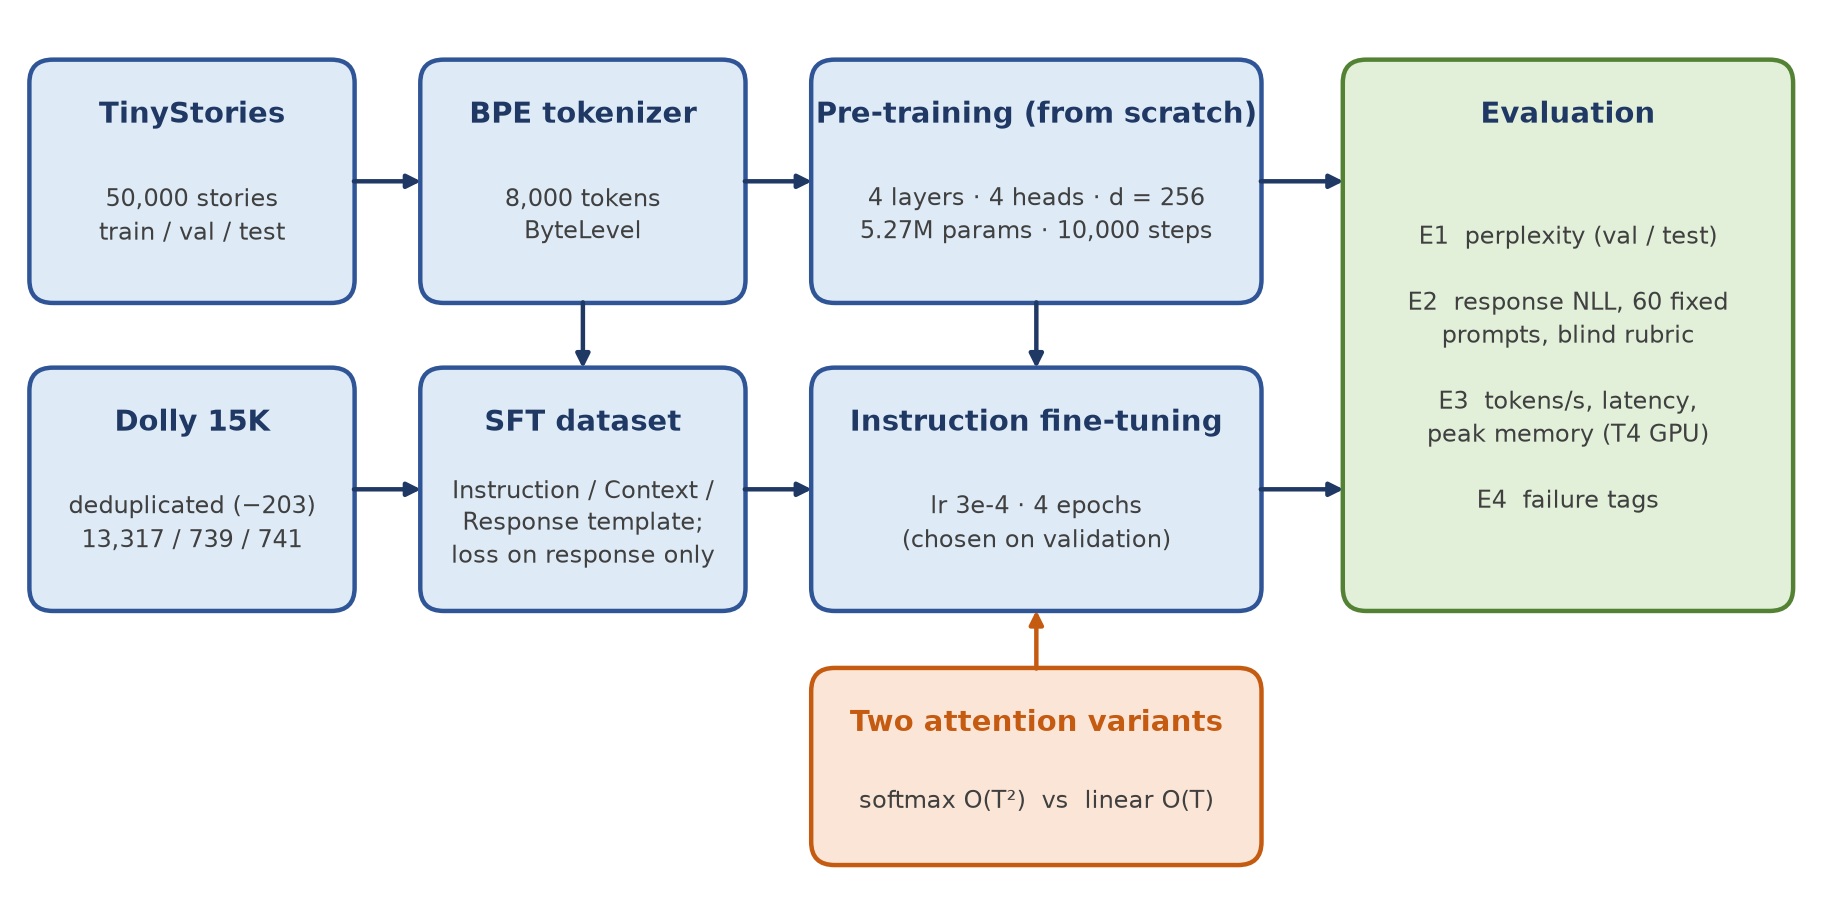
\includegraphics[width=\columnwidth]{pipeline.png}
\caption{Pipeline. The two attention variants share data, tokenizer, training engine and evaluation.}
\label{fig:pipeline}
\end{figure}

\subsection{Training}
Pre-training uses AdamW~\cite{adamw} (learning rate $3\times10^{-4}$, weight decay 0.1, 200 warm-up steps) with batch
32 for 10{,}000 steps, about six passes over the sample. The same seed, data order and GPU are used for both
variants. Fine-tuning continues from each pre-trained checkpoint for 4 epochs at batch 4 (10{,}700 steps). We chose
the learning rate on Dolly validation in a short rehearsal: after one epoch, $2\times10^{-5}$, $10^{-4}$ and
$3\times10^{-4}$ gave response NLL 5.34, 4.84 and 4.64.

\subsection{Evaluation}
\textbf{E1:} token-weighted NLL and perplexity on held-out stories.
\textbf{E2:} response-only NLL on the Dolly test split, plus 60 fixed held-out prompts (balanced across categories)
decoded greedily for 128 tokens with identical settings for every model. We report stopping rate, 4-gram repetition,
prompt copying and ROUGE-L~\cite{rouge}, and score the 120 outputs (60 prompts, two models) on a blind 0--2 rubric
for relevance, format, answering rather than echoing, and coherence. The outputs were shuffled and the model labels
hidden. The rubric was scored by an automated LLM judge, not by human raters (Section~\ref{sec:limits}).
\textbf{E3:} training throughput, forward latency for $T=128$ to $2{,}048$ and peak memory, with CUDA-synchronised
timing, discarded warm-up and medians of repeated runs.

\section{Results}
\subsection{E1: Pre-training}
Validation loss falls steadily and is still falling at step 10{,}000 (Fig.~\ref{fig:val}). The best checkpoint is
the last one, so there is no sign of overfitting after six passes. The standard model reaches validation perplexity
8.60 and test perplexity 8.51 against 8{,}000 for a uniform guess (Table~\ref{tab:main}). Continuations are fluent
TinyStories prose but not always consistent: in one, a monster is ``big and scary'' and in the next sentence ``very
friendly''.

\begin{figure}[t]
\centering
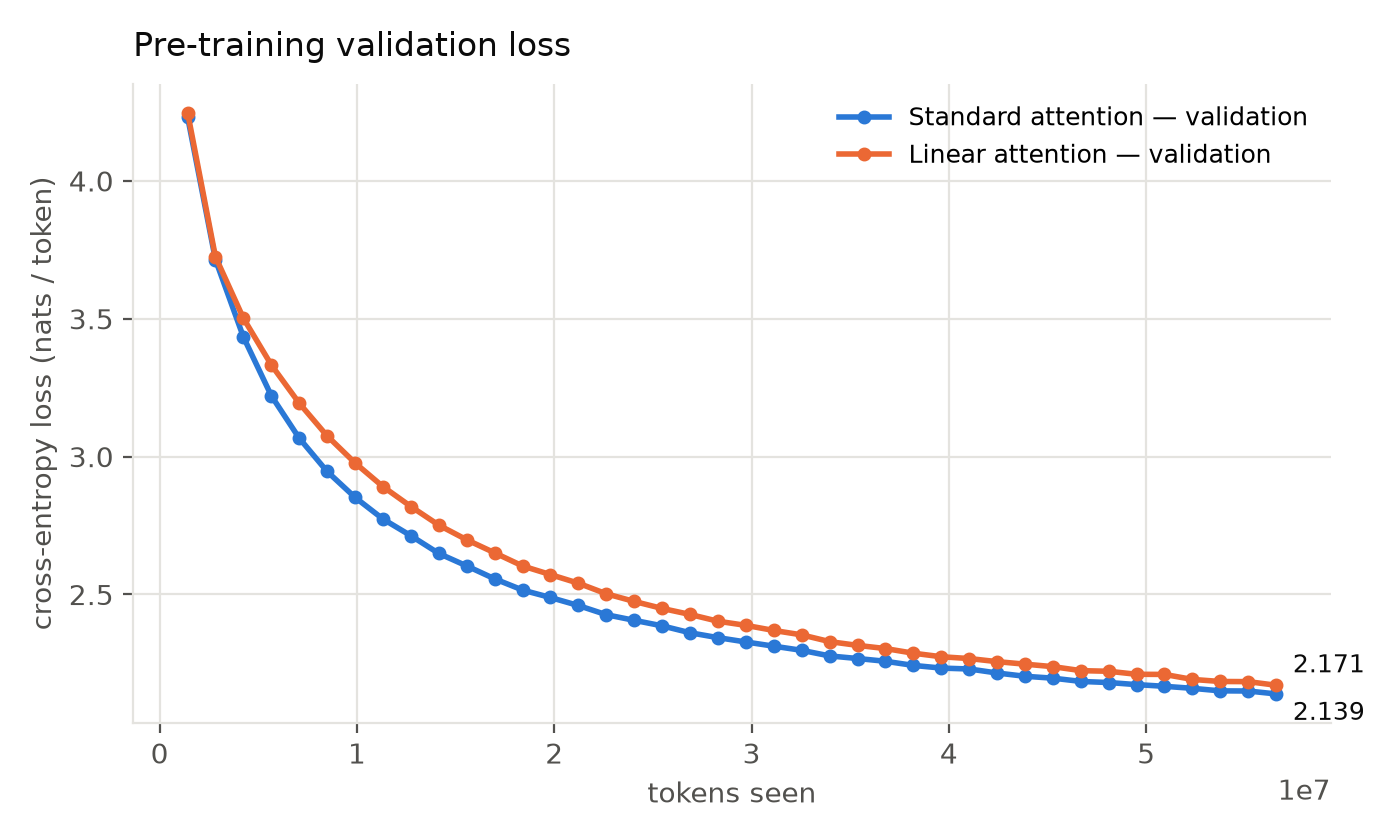
\includegraphics[width=\columnwidth]{pretrain_val_loss.png}
\caption{Pre-training validation loss, both attention variants. Linear attention stays slightly above softmax
attention throughout; both are still improving at 10{,}000 steps.}
\label{fig:val}
\end{figure}

\begin{table}[t]
\centering
\caption{Final results (Tesla T4, 10{,}000 pre-training steps, seed 42).}
\label{tab:main}
\begin{tabular}{@{}lrr@{}}
\toprule
 & Softmax & Linear \\
\midrule
Test perplexity (uniform 8{,}000) & \textbf{8.51} & 8.78 \\
Pre-training time & \textbf{1{,}419 s} & 3{,}319 s \\
Dolly test response NLL after SFT & \textbf{3.93} & 4.11 \\
Fine-tuning time & \textbf{305 s} & 532 s \\
Throughput, batch $32\times256$ (tokens/s) & \textbf{79{,}198} & 29{,}471 \\
Peak training memory, batch $32\times256$ & \textbf{1.9 GB} & 4.5 GB \\
\bottomrule
\end{tabular}
\end{table}

\subsection{E2: Instruction fine-tuning}
Fine-tuning lowers response NLL on the Dolly test split from 6.38 to 3.93 (response perplexity 589 to 51), and
validation loss was still falling after four epochs. Table~\ref{tab:sft} compares the two models on the 60 fixed
prompts. The pre-trained model answers 45 of the 60 prompts with a children's story; after fine-tuning none are
stories, outputs stop on their own more often, and overlap with the reference answers rises. The rubric total roughly
doubles, but almost all of the gain is in relevance and format. Coherence is unchanged, because looping answers
replace looping stories. The ``answers'' score falls, because a story still counts as new content while fine-tuned
outputs often echo the question (``A landlord is a landlord that is a landlording.'').

Greedy decoding makes the fine-tuned model loop: 32 of 60 outputs have 4-gram repetition above 0.5, against 11
before fine-tuning. Loss is computed with the true previous tokens, whereas greedy decoding feeds the model its own
output, so one repeated phrase makes itself more likely~\cite{holtzman}. Sampling (temperature 0.8, top-$k$ 50)
reduces looping to 1 of 60 and raises the stopping rate to 90\%, but does not make the answers correct. The best of
the 60 fine-tuned answers is partly right (``Kora is string, Colora is percussion''); most are fluent and wrong.

\begin{table}[t]
\centering
\caption{E2 on 60 held-out Dolly prompts, greedy decoding. Rubric criteria are 0--2, total out of 8.}
\label{tab:sft}
\begin{tabular}{@{}lrr@{}}
\toprule
 & Pre-trained & Fine-tuned \\
\midrule
Response NLL (full test split) & 6.38 & \textbf{3.93} \\
Rubric total / 8 & 1.25 & \textbf{2.60} \\
\quad relevance / format & 0.07 / 0.02 & \textbf{0.90 / 0.80} \\
\quad answers / coherence & \textbf{0.78} / 0.38 & 0.52 / 0.38 \\
Story-like answers & 45 / 60 & \textbf{0 / 60} \\
Stops on its own (EOS rate) & 0.33 & \textbf{0.55} \\
Outputs with 4-gram repetition $>0.5$ & \textbf{11 / 60} & 32 / 60 \\
ROUGE-L vs reference & 0.078 & \textbf{0.139} \\
\bottomrule
\end{tabular}
\end{table}

\subsection{E3: Softmax vs linear attention}
Linear attention was slower and heavier at every size we measured: 0.35--0.40$\times$ the training throughput and
2.2--2.5$\times$ the peak memory of softmax attention, a gap far larger than the run-to-run spread (standard deviation
about 1\% over four identical runs). Its scaling, however, matches the theory (Fig.~\ref{fig:lat}). Each doubling of
$T$ multiplies softmax forward time by 2.03, rising to 2.95, while linear attention stays at about 2.0. The latency
ratio therefore shrinks from 2.52$\times$ at 128 tokens to 1.08$\times$ at 2{,}048. The reason is the constant factor:
the causal linear form keeps a $64\times64$ state (4{,}096 numbers) per token and head, while softmax attention keeps
$T$ scores, so below about 4{,}000 tokens the linear form moves more data. At equal steps, linear attention also ended
3.1\% worse in test perplexity and 0.18 nats worse in response NLL after fine-tuning; this gap shrank from 9\% at
3{,}000 steps in our rehearsal.

\begin{figure}[t]
\centering
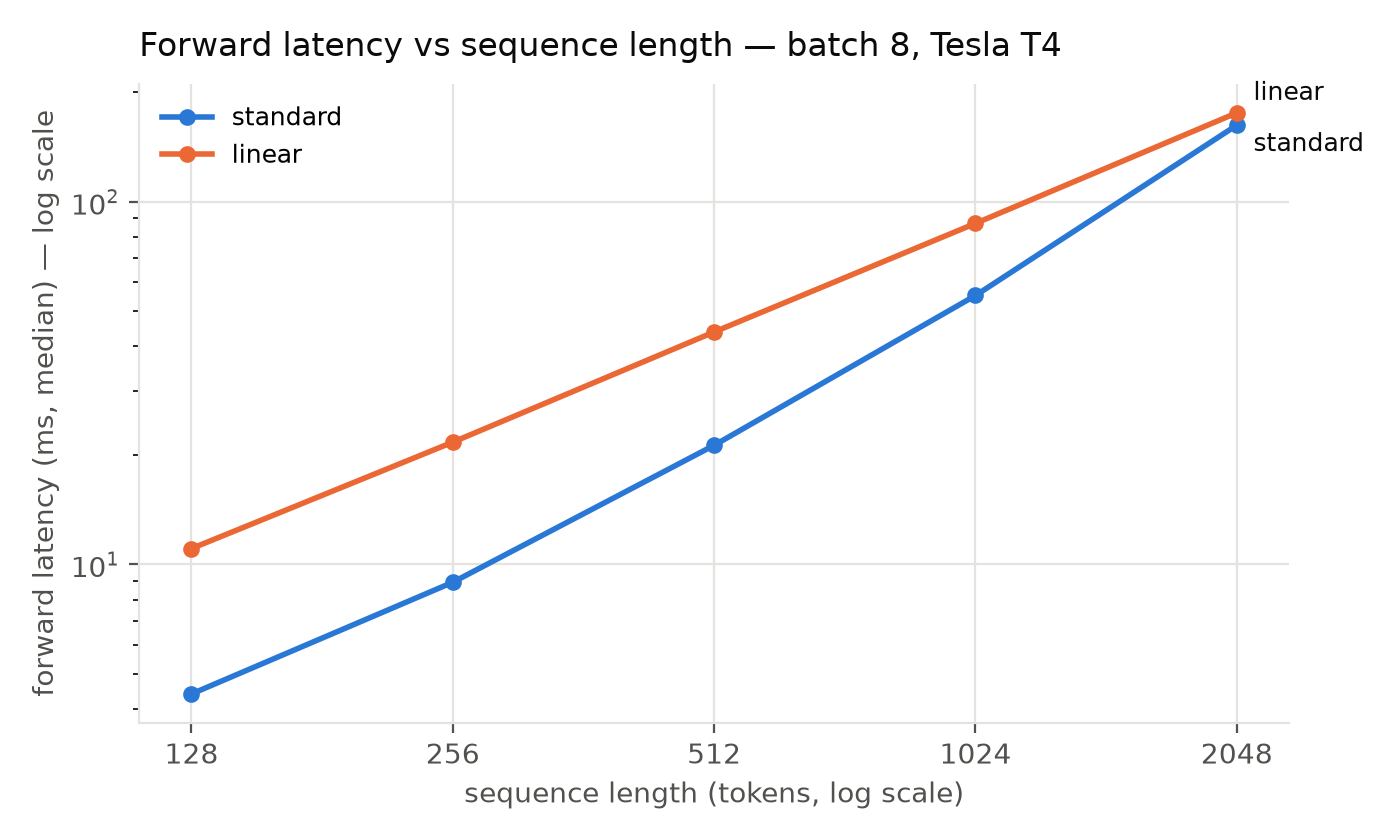
\includegraphics[width=\columnwidth]{bench_t4_forward_latency.png}
\caption{Forward latency against sequence length (batch 8, log--log). Linear attention grows linearly but starts
2.5$\times$ higher and only approaches softmax attention at 2{,}048 tokens.}
\label{fig:lat}
\end{figure}

\subsection{E4: Failure analysis}
The failure tags from the rubric pass show four patterns. \emph{Story mode} (45/60 pre-trained, 0/60 fine-tuned):
the pre-training data contains only stories. \emph{Loops} (38/60 and 40/60 by the rubric's repeated-phrase rule):
greedy decoding without a repetition penalty. \emph{Echo} (0/60 and 8/60): the fine-tuned model opens with the
question's subject but has nothing to add. \emph{Factual errors} (12/60 fine-tuned): a 5M-parameter model trained on
children's stories holds almost no world knowledge, and fine-tuning on 13K examples does not supply it.

\section{Limitations}\label{sec:limits}
We ran one seed per configuration. The rubric was scored by a single automated LLM judge rather than human raters,
and its blinding was partial because the same judge had read a few labelled outputs while the results were written
up; it confirms, rather than replaces, the automatic measures. About 20\% of Dolly prompts do not fit a 256-token
context, which under-represents long-context tasks such as summarisation. Both models were still improving when
training stopped. Efficiency results describe our implementation: a chunked or fused kernel, recurrent decoding or a
KV cache would change the constants.

\section{Conclusion}
Pre-training from scratch on a free GPU works: test perplexity fell from 8{,}000 to 8.5 in 24 minutes. Instruction
fine-tuning lowered response loss and taught the model the form of an answer, but not its content, and greedy
decoding exposed loops that the loss did not show. Linear attention scaled as theory predicts but was slower, heavier
and slightly worse at the context lengths a model of this size uses; at 256 tokens, softmax attention is the better
choice.

\section*{Contributions}
\textbf{Akash Shivanand Bagoji:} model, both attention variants, training engine, pre-training.
\textbf{Haneesh Elamati:} preprocessing, deduplication, tokenizer, datasets, response-only fine-tuning.
\textbf{Samvith Vaddiparthi:} evaluation, benchmarks, rubric aggregation, failure analysis, report.
Code, data links and all results: \url{https://github.com/akashsb2005/AFML-Project}.

\begin{thebibliography}{9}
\bibitem{vaswani} A.~Vaswani et al., ``Attention is all you need,'' in \emph{Proc. NeurIPS}, 2017.
\bibitem{katharopoulos} A.~Katharopoulos, A.~Vyas, N.~Pappas, and F.~Fleuret, ``Transformers are RNNs: Fast
autoregressive transformers with linear attention,'' in \emph{Proc. ICML}, 2020.
\bibitem{tinystories} R.~Eldan and Y.~Li, ``TinyStories: How small can language models be and still speak coherent
English?'' arXiv:2305.07759, 2023.
\bibitem{dolly} M.~Conover et al., ``Free Dolly: Introducing the world's first truly open instruction-tuned LLM,''
Databricks, 2023.
\bibitem{ouyang} L.~Ouyang et al., ``Training language models to follow instructions with human feedback,'' in
\emph{Proc. NeurIPS}, 2022.
\bibitem{adamw} I.~Loshchilov and F.~Hutter, ``Decoupled weight decay regularization,'' in \emph{Proc. ICLR}, 2019.
\bibitem{holtzman} A.~Holtzman, J.~Buys, L.~Du, M.~Forbes, and Y.~Choi, ``The curious case of neural text
degeneration,'' in \emph{Proc. ICLR}, 2020.
\bibitem{rouge} C.-Y.~Lin, ``ROUGE: A package for automatic evaluation of summaries,'' in \emph{Text Summarization
Branches Out}, 2004.
\end{thebibliography}

\end{document}
